\subsection{CU20 Visualizar Solicitudes}
En esta pantalla, el administrador podrá visualizar en una tabla cada una de las solicitudes de refacción que los empleados han hecho. Esta tabla consta de tres columnas, la primera es el número de Inventario de la refacción, la segunda es el nombre del empleado que solicitó la refacción y la tercera es una descripción de la refacción. Solo consta de tres opciones en la parte inferior de la ventana:
\begin{itemize}
	
	\item \textbf{Atender Solicitud:} En esta opción se desplegará una pantalla donde el administrador podrá verificar la solicitud y aceptarla. En caso de que no se elija una fila de la tabla, se mostrará un mensaje de error en pantalla. (Figura \ref{fig:Alerta Solicitudes - Vista de Escenarios}).
	\item \textbf{Salir:} Regresará a la pantalla anterior la cual es el Menú del administrador (figura \ref{fig:Pantalla Visualizar Menu Administrador - Vista de Escenarios}).
\end{itemize}
\begin{figure}[!h]
	\centering
	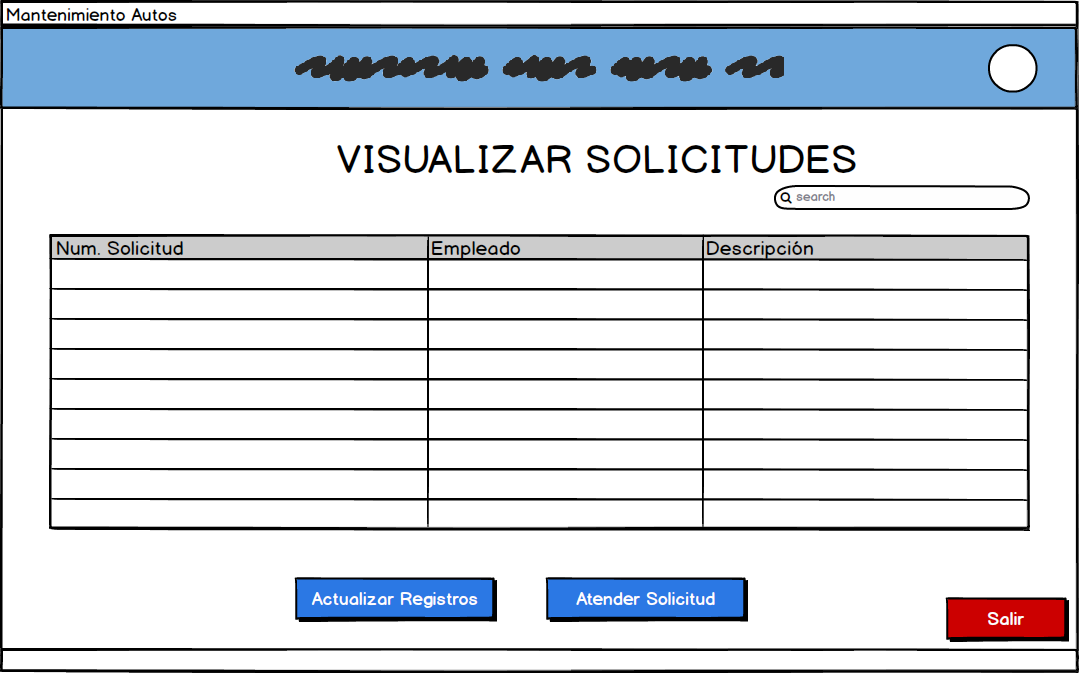
\includegraphics[width=0.8\textwidth]{./diseno/vescenarios/imagenes/visualizarSolicitudes}
	\caption{Pantalla Visualizar Solicitudes - Vista de Escenarios}
	\label{fig:Pantalla Visualizar Solicitudes- Vista de Escenarios}
\end{figure}
\begin{figure}[!h]
	\centering
	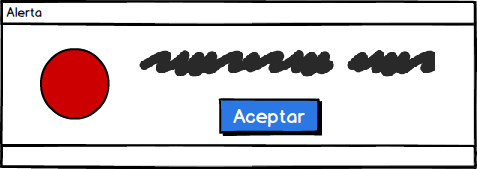
\includegraphics[width=0.3\textwidth]{./diseno/vescenarios/imagenes/alerta}
	\caption{Alerta Solicitudes- Vista de Escenarios}
	\label{fig:Alerta Solicitudes - Vista de Escenarios}
\end{figure}
\clearpage